\documentclass{beamer}
\usepackage[utf8]{inputenc}

\usetheme{Madrid}
\usecolortheme{default}
\usepackage{extarrows}
\usepackage{amsmath}
\usepackage{extarrows}
\usepackage{amssymb,amsfonts,amsthm}
\usepackage{txfonts}
\usepackage{tkz-euclide}
\usepackage{listings}
\usepackage{adjustbox}
\usepackage{array}
\usepackage{tabularx}
\usepackage{gvv}
\usepackage{lmodern}
\usepackage{circuitikz}
\usepackage{tikz}
\usepackage{graphicx}
\usepackage{amsmath} 

\setbeamertemplate{page number in head/foot}[totalframenumber]

\usepackage{tcolorbox}
\tcbuselibrary{minted,breakable,xparse,skins}

\definecolor{bg}{gray}{0.95}
\DeclareTCBListing{mintedbox}{O{}m!O{}}{%
  breakable=true,
  listing engine=minted,
  listing only,
  minted language=#2,
  minted style=default,
  minted options={%
    linenos,
    gobble=0,
    breaklines=true,
    breakafter=,,
    fontsize=\small,
    numbersep=8pt,
    #1},
  boxsep=0pt,
  left skip=0pt,
  right skip=0pt,
  left=25pt,
  right=0pt,
  top=3pt,
  bottom=3pt,
  arc=5pt,
  leftrule=0pt,
  rightrule=0pt,
  bottomrule=2pt,
  toprule=2pt,
  colback=bg,
  colframe=orange!70,
  enhanced,
  overlay={%
    \begin{tcbclipinterior}
    \fill[orange!20!white] (frame.south west) rectangle ([xshift=20pt]frame.north west);
    \end{tcbclipinterior}},
  #3,
}
\lstset{
    language=C,
    basicstyle=\ttfamily\small,
    keywordstyle=\color{blue},
    stringstyle=\color{orange},
    commentstyle=\color{green!60!black},
    numbers=left,
    numberstyle=\tiny\color{gray},
    breaklines=true,
    showstringspaces=false,
}
\title %optional
{4.7.24}
\date{September 12 ,2025}

\author 
{Kartik Lahoti - EE25BTECH11032}

\begin{document}


\frame{\titlepage}
\begin{frame}{Question}
Find the equation of line passing through the point $\brak{5,2}$ and perpendicular to the line joining the points $\brak{2,3}$ and $\brak{3,-1}$
\end{frame}

\begin{frame}{Theoretical Solution}

Given : 
\begin{table}[H]
    \centering
    \begin{tabular}{|c|c|}
\hline
\textbf{Name} & \textbf{Value} \\ \hline
$\vec{A}$ & $\myvec{2 & 1 \\0 & 3}$ \\ \hline
\end{tabular}

    \caption{4.7.24}
    \label{tab:placeholder_1}
\end{table}

Let , $\vec{X}$ be a vector on the Required Line

\end{frame}
\begin{frame}{Theoretical Solution}
Direction Vector for the Line $\vec{AB}$ , 
\begin{align}
    \vec{B} - \vec{A} = \myvec{3 \\ -1} - \myvec{2 \\ 3} = \myvec{1 \\ -4}
\end{align}

Direction Vector for the Required Line in terms of $\vec{X}$ , 

\begin{align}
    \vec{X} - \vec{P} = \brak{\vec{X} - \myvec{5 \\ 2}}
\end{align}

\end{frame}
\begin{frame}{Theoretical Solution}
Direction Vector for the Line $\vec{AB}$ is perpendicular to the required line
\begin{align}
        \therefore \brak{\vec{B} - \vec{A}}^{\top}\brak{\vec{X} - \myvec{5 \\ 2}} &= 0
\end{align}
\begin{align}
    \myvec{1 & -4}\brak{\vec{X} - \myvec{5 \\ 2}} &= 0
\end{align}
\end{frame}

\begin{frame}{Theoretical Solution}
Hence, the desired equation is 

\begin{align}
    \myvec{1 & -4}\vec{X} = -3
\end{align}
\end{frame}

\begin{frame}[fragile]
    \frametitle{C Code (1)}

    \begin{lstlisting}
double dot_prod(double *A , double *B , int m )
{
    double sum = 0.0 ; 
    for ( int i = 0 ; i < m ; i++ )
    {
        sum += A[i]*B[i] ;     
    }
    return sum; 
}
    \end{lstlisting}
\end{frame}

\begin{frame}[fragile]
    \frametitle{C Code (2) - Function to Generate Points on Line}
    \begin{lstlisting}
    
void linegen(double *XY, double *A , double *B , int n , int m )
{
    double temp[m] ; 
    for (int i = 0 ; i < m ; i++)
    {
        temp [ i ] = (B[i]- A[i]) /(double) n ; 
    }
    for (int i = 0 ; i < n ; i++ )
        for (int j = 0 ; j < m ; j++)
            XY[j*n + i ] = A[j] + temp[j] * i ; 
           
}

\end{lstlisting}
\end{frame}

\begin{frame}[fragile]
    \frametitle{Python Code - Using Shared Object}
    \begin{lstlisting}
import ctypes as ct
import numpy as np
import matplotlib.pyplot as plt

handc1 = ct.CDLL("./func.so")

handc1.dot_prod.argtypes = [
    ct.POINTER(ct.c_double),
    ct.POINTER(ct.c_double),
    ct.c_int
]

handc1.dot_prod.restype = ct.c_double

\end{lstlisting}
\end{frame}

\begin{frame}[fragile]
    \frametitle{Python Code - Using Shared Object}
    \begin{lstlisting}

A = np.array([2,3], dtype= np.float64).reshape(-1,1)
B = np.array([3,-1] , dtype= np.float64 ).reshape(-1,1)
P = np.array([5,2] , dtype= np.float64 ).reshape(-1,1)
K = (B-A) 
const = handc1.dot_prod(
    K.ctypes.data_as(ct.POINTER(ct.c_double)),
    P.ctypes.data_as(ct.POINTER(ct.c_double)),
    2
)
K = K.reshape(1,-1)
print("Required Line Equation : ")
print(K,"X = ", const )

\end{lstlisting}
\end{frame}

\begin{frame}[fragile]
    \frametitle{Python Code - Using Shared Object}
    \begin{lstlisting}
def line_cre(P: np.ndarray , Q: np.ndarray, str1 , str2):
    handc2 = ct.CDLL("./line_gen.so")

    handc2.linegen.argtypes = [
        ct.POINTER(ct.c_double),
        ct.POINTER(ct.c_double),
        ct.POINTER(ct.c_double),
        ct.c_int , ct.c_int
    ]
    
\end{lstlisting}
\end{frame}
\begin{frame}[fragile]
    \frametitle{Python Code - Using Shared Object}
    \begin{lstlisting}
    
handc2.linegen (
        XY.ctypes.data_as(ct.POINTER(ct.c_double)),
        P.ctypes.data_as(ct.POINTER(ct.c_double)),
        Q.ctypes.data_as(ct.POINTER(ct.c_double)),
        n,2
    )
    plt.plot(XY[0,:],XY[1,:], str1 , label = str2 )
    
    \end{lstlisting}
\end{frame}

\begin{frame}[fragile]
    \frametitle{Python Code - Using Shared Object}
    \begin{lstlisting}
plt.figure()
#the ratio of perp on Line Ab is 7:10 
line_cre(P,(10 * A+ 7 * B)/17,"g-","Required Line")
line_cre(A,B,"r--" , "Line AB")

coords = np.block([[A,B,P, (10 * A+ 7 * B)/17 ]])
plt.scatter(coords[0,:],coords[1,:])
vert_labels = ['A','B','P','Q']

for i, txt in enumerate(vert_labels):
    plt.annotate(f'{txt}\n({coords[0,i]:.1f}, {coords[1,i]:.1f})',
                 (coords[0,i], coords[1,i]),
                 textcoords="offset points",
                 xytext=(25,-12),
                 ha='center', va = 'bottom')
\end{lstlisting}
\end{frame}

\begin{frame}[fragile]
    \frametitle{Python Code - Using Shared Object}
    \begin{lstlisting}
plt.xlabel('$x$')
plt.ylabel('$y$')
plt.legend(loc='best')
plt.grid()

plt.title("Fig:4.7.24")
plt.axis('equal')

plt.savefig("../figs/perpbisector1.png")
plt.show()

#plt.savefig('../figs/perpbisector1.png')
#subprocess.run(shlex.split("termux-open ../figs/perpbisector1.png"))

\end{lstlisting}
\end{frame}

\begin{frame}[fragile]
    \frametitle{Python Code}
    \begin{lstlisting}
import math
import sys
sys.path.insert(0, '/home/kartik-lahoti/matgeo/codes/CoordGeo')
import numpy as np
#import numpy.linalg as LA
import matplotlib.pyplot as plt

from line.funcs import *

#if using termux
#import subprocess
#import shlex
\end{lstlisting}
\end{frame}

\begin{frame}[fragile]
    \frametitle{Python Code }
    \begin{lstlisting}
A = np.array([2,3]).reshape(-1,1)
B = np.array([3,-1]).reshape(-1,1)
P = np.array([5,2]).reshape(-1,1)
K = (B-A).T

x = np.dot(K,P)
x = np.squeeze(x)
print("Required Line Equation : ")
print(K,"X = ", x )
\end{lstlisting}
\end{frame}

\begin{frame}[fragile]
    \frametitle{Python Code }
    \begin{lstlisting}
def plot_it(P,Q,str1, str2):
    x_l = line_gen_num(P,Q,20)
    plt.plot(x_l[0,:],x_l[1,:] ,str1 , label = str2 )

plt.figure()

plot_it(P,(10 * A+ 7 * B)/17,"g-","Required Line")
plot_it(A,B,"r--" , "Line AB")


\end{lstlisting}
\end{frame}

\begin{frame}[fragile]
    \frametitle{Python Code }
    \begin{lstlisting}

coords = np.block([[A,B,P, (10 * A+ 7 * B)/17 ]])
plt.scatter(coords[0,:],coords[1,:])
vert_labels = ['A','B','P','Q']

for i, txt in enumerate(vert_labels):
    plt.annotate(f'{txt}\n({coords[0,i]:.1f}, {coords[1,i]:.1f})',
                 (coords[0,i], coords[1,i]),
                 textcoords="offset points",
                 xytext=(25,-12),
                 ha='center', va = 'bottom')
    \end{lstlisting}
\end{frame}
\begin{frame}[fragile]
    \frametitle{Python Code }
    \begin{lstlisting}
plt.xlabel('$x$')
plt.ylabel('$y$')
plt.legend(loc='best')
plt.grid()

plt.title("Fig:4.7.24")
plt.axis('equal')

plt.savefig("../figs/perpbisector2.png")
plt.show()

#plt.savefig('../figs/perpbisector2.png')
#subprocess.run(shlex.split("termux-open ../figs/perpbisector2.png"))
    \end{lstlisting}
\end{frame}


\begin{frame}{Plot}
    \centering
    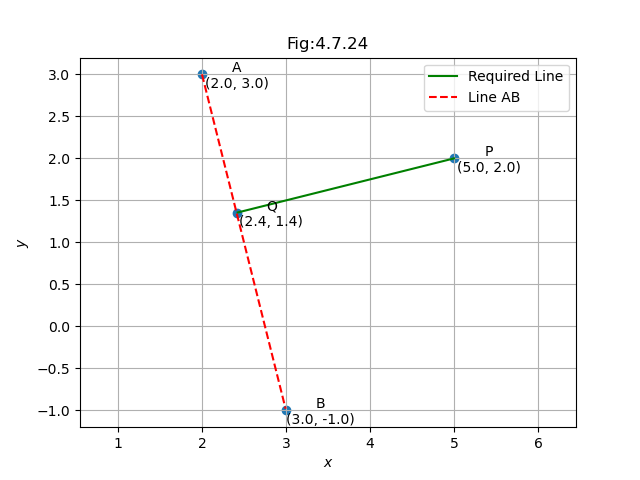
\includegraphics[width=\columnwidth, height=0.8\textheight, keepaspectratio]{../figs/perpendicular1.png}   
\end{frame}


\end{document}
